\Titre{Firewalls}
\usepackage{ifthen}


\def\txthl#1{ \ifthenelse{\lengthtest{#1 pt<0.5pt}}{\top}{\bot} }

\begin{document}

\begin{reveals}
                
\maketitle


\section{NAT}

\begin{frame}[c]{Context}
  
  \begin{block}{Local Area Network (LAN)}
    \begin{itemize}
    \item closed network without direct access to Internet
    \item Most people work only in this kind of networks
    \item Examples: \textit{eduroam}, \emph{ups}, etc.
    \end{itemize}
  \end{block}

  \vfill

  \begin{block}{Border with the Internet}
    \begin{itemize}
    \item One computer is tasked with managing the interface between a
      LAN and:
      \begin{itemize}
      \item a greater LAN, or
      \item the Internet
      \end{itemize}
    \item The control of the border is the task of a \emph{firewall}
    \end{itemize}
  \end{block}

  \vfill

  \begin{block}{Firewall description}
    \begin{itemize}
    \item is part of the Operating System
    \item has direct access to all the communications and all the
      network interface cards
    \item issues \emph{judgements} on what to do to TCP/IP-level messages
    \end{itemize}
  \end{block}

\end{frame}

\begin{frame}{Exercice: Separation in a Network}

  \begin{block}{Situation}
    A company has an \textit{e}commerce web site. Some of its
    employees are connected using an ethernet network, some use wifi,
    and some are remotely connected. Among the employees, there are
    developers, administrators, and users. In addition to its locally
    run Web server, the company has internal servers (DNS, DB server,
    Business-related application servers). Finally, clients visiting
    the company may use the wifi to connect to the Web.
  \end{block}

  \vfill
  \begin{block}{Questions}
    \begin{enumerate}
    \item List the components and their network connections. The
      current network is represented by a single component, a
      \emph{bus}.
    \item We want to install a firewall to protect the assets of the
      company. Which components must still be accessible from the
      outside ?
    \item What happens if a hacker can take control of the Web server
      ?
    \item Propose a separation of the components into disjoint zones
      (disregard wifi for the moment). How can you implement this
      separation?
    \item What happens when one adds the wifi network?
    \end{enumerate}
  \end{block}

\end{frame}



\section{Border Control with a Firewall}

\subsection{Packet Selection}


\begin{frame}[c]{Common structure}
  
  \begin{center}
    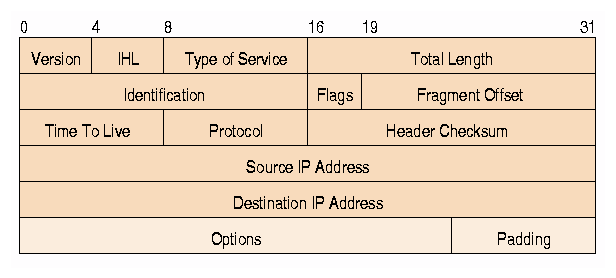
\includegraphics[height=0.5\textheight]{images/ipcomplete.png}
  \end{center}
\end{frame}


\begin{frame}[c]{Addresses}
  
  \begin{center}
    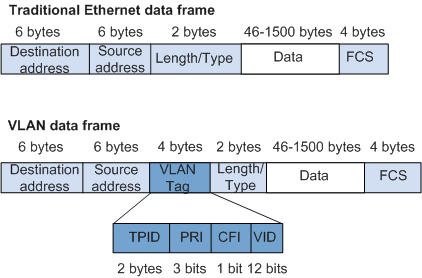
\includegraphics[height=0.5\textheight]{images/ipframe.png}
  \end{center}

  \begin{block}{IP crash course}
    A packet of the IP protocol has:
    \begin{itemize}
    \item a \emph{source} IP address, selected by iptables with
      \texttt{-s 192.168.0.3}
    \item a \emph{destination} IP address, selected by iptables with
      \texttt{-d 192.168.0.3}
    \end{itemize}
  \end{block}
\end{frame}


\begin{frame}[c]{Interfaces}
  
  \begin{block}{Physical devices}
      \begin{itemize}
      \item recognized by the OS: \texttt{eth0}
      \item Virtual LAN (VLAN): peripheral annotated with a
        \emph{mark} (a number \(0\le n< 4096\)), \textit{e.g.} \texttt{eth0.123}
      \end{itemize}
  \end{block}

  \vfill

  \begin{block}{Iptables}
    Refers to a device with its name, and whether it:
    \begin{itemize}
    \item inputs a message: \texttt{-i eth0.20} selects the packets
      with the mark 20 incoming in device \texttt{eth0}
    \item outputs a message: \texttt{-o eth1.30} selects the packets
      with the mark 30 going out through the device \texttt{eth1}
    \end{itemize}
    
  \end{block}
\end{frame}

\begin{frame}
  \frametitle{Protocol and Port}
  \vfill
  \begin{block}{Protocol}
    \begin{itemize}
    \item \textbf{tcp}, \textbf{udp},icmp, or other listed in
      (\texttt{/etc/protocols})
    \item Most often one wants to select tcp: \texttt{-p tcp}
    \end{itemize}
  \end{block}
  \vfill
  \begin{block}{Port}
    \begin{itemize}
    \item source port or destination port
    \item one has to use a protocol that understands \emph{ports}, like TCP
    \item for iptables, a port can have a name defined in
      \texttt{/etc/services}
    \item Examples: \texttt{-sport 80}, \texttt{-dport smtp}
    \end{itemize}
  \end{block}
  \vfill
\end{frame}


\begin{frame}[c]{Position in request/response}
  \begin{block}{Underlying issue}
    \begin{itemize}
    \item we often want to discard all incoming messages on an
      interface
    \item also, we still want to allow responses to a request we have accepted
    \item Conclusion: remember (in a state) which messages have been
      sent to whom, and allow the responses
    \end{itemize}
  \end{block}
  \vfill
  \begin{block}{Module \texttt{state/conntrack}}
    \begin{itemize}
    \item \texttt{-m state} or \texttt{-m conntrack} to be able to specify a state
    \item \texttt{--state} to say which states are selected
    \item marche pour tcp \textbf{et} udp
    \end{itemize}
  \end{block}
  \vfill
  \begin{block}{Main states}
    \begin{itemize}
    \item \texttt{new}: new connection
    \item \texttt{established}: response to a previous message
    \item \texttt{related}: related to an existing previous message
      (\emph{e.g.} when the destination port change)
    \end{itemize}
  \end{block}

\end{frame}

\subsection{Packet Handling}



\begin{frame}
  \frametitle{Architecture}

  \vfill
  \begin{center}
    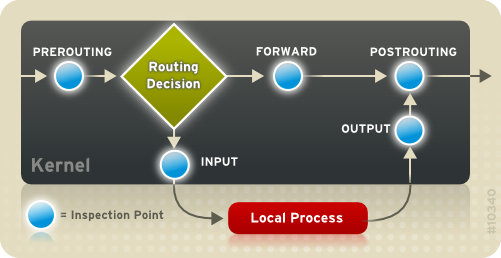
\includegraphics[width=0.8\linewidth]{images/iptables_small}
  \end{center}
  \vfill
\end{frame}

\begin{frame}[c]{Tables (iptables)}

  \begin{block}{Organisation}
    \begin{itemize}
    \item Rules are organized per \emph{tables}
    \item The default table is \emph{filter}, which is employed for
      access control, to decide whether a packet can go through
    \end{itemize}
  \end{block}

  \vfill

  \begin{block}{Non-default table}
    to use another table, use \texttt{-t name} where \texttt{name} is:
    \begin{description}
    \item[mangle:] to alter packets
    \item[nat:] for connecting a LAN with a wider network
    \item[security:] for Mandatory Access Control with SELinux
    \end{description}
    one can also create new tables, and send packets to these tables
    for closer examination
  \end{block}

\end{frame}


\begin{frame}[c]{Chains}

  \begin{block}{Chains in the filter table}
    A \emph{chain} process a message according to its origin and
    destination:
    \begin{description}
    \item[INPUT chain:] the message is directed to a program on this machine
    \item[OUTPUT chain:] the message was sent by a program on this machine
    \item[FORWARD chain:] (border) the message comes from another
      machine and goes to another machine
    \end{description}
  \end{block}

  \begin{block}{Rules and chains}
    \begin{itemize}
    \item A chain is a \textcolor{red}{list of rules}
    \item Rules can be inserted (\texttt{-I chain}) or appended
      (\texttt{-A chain}) to the chain
    \item The first rule matching a packet is applied
    \item Rules are usually added with \texttt{-A}
    \end{itemize}
  \end{block}

  
\end{frame}


\begin{frame}[c]{Rules}
  
  \begin{block}{Rules for rules}
    \begin{itemize}
    \item Each rule belongs to a chain
    \item Each chain belongs to a table
    \item We have so far seen how to decide whether a rule is
      applicable on a packet
    \item When it is, the rule issues a \textbf{judgement} on the
      selected packet is specified with \texttt{-j}
    \end{itemize}
  \end{block}

  \vfill
  \begin{block}{Possible judgements}
    \begin{description}
    \item[ACCEPT:] stop the filtering and let the packet go
    \item[DROP:] stop the filtering and discard the packet
    \item[REJECT:] stop the filtering and inform the source address
      that the packet has been discarded
    \item[chain name:] the packet is sent to another chain for further processing
    \end{description}
  \end{block}
\end{frame}

\begin{frame}
  \frametitle{Examples}
  \vfill
  \begin{block}{Goal}
    The outside is connected to \texttt{eth1} and must be prevented
    from using the local network (on \texttt{eth0})
  \end{block}
  \pause\vfill 
  \begin{block}{First version}
    \small\tt iptables -I FORWARD -i eth1 -o eth0 -j REJECT
  \end{block}
   \pause\vfill 
 \begin{block}{Second version }
    \small\tt iptables -I FORWARD -m state -\,-state NEW -i eth1 -o eth0 -j REJECT
  \end{block}
   \pause\vfill 
 \begin{block}{Authorize one specific connection (if not rejected before}
   \small\tt iptables -I FORWARD -i eth1 -d 10.0.0.2 -j ACCEPT
  \end{block}
  \vfill
\end{frame}

\begin{frame}[c,fragile]{Logging packets}
  
  \begin{block}{Routing to another chain}
    \begin{itemize}
    \item A packet can be sent to another chain for further processing
    \item It can also be sent to a special chain: \texttt{LOG}
    \end{itemize}
  \end{block}

  \vfill

  \begin{block}{Goal and properties}
    \begin{itemize}
    \item The routing to \texttt{LOG} doesn't stop the processing in
      the current chain
    \item The kernel records the event in \url{/var/log/syslog}
    \item Using \texttt{-j LOG --log-prefix='[iptables] '} allows for
      easily finding the events in the log
    \item One can specify a own file for these (in \url{/etc/rsyslog.d/00-my\_iptables.conf}):
\begin{verbatim}
:msg,contains,"[iptables] " -/var/log/iptables.log
& stop
\end{verbatim}
    \end{itemize}
  \end{block}

\end{frame}

\begin{frame}
  \frametitle{The NAT Table}
  \vfill
  \begin{block}{LAN and NAT}
    \begin{itemize}
    \item LAN use \emph{reserved} addressed (defined in the IP
      protocol)
    \item These addresses are not valid (cannot be contacted) on the Internet
    \item Impact on Security:
      \begin{itemize}
      \item Allow machines on the LAN to connect to the Internet
      \item Forbid machines on the Internet to connect to machines in
        the LAN
      \end{itemize}
    \item Employed by Eduroam, Universities, ISP, etc.
    \item Works on the \texttt{PREROUTING} (before \texttt{INPUT}),
      \texttt{OUTPUT}, and \texttt{POSTROUTING} (after
      \texttt{OUTPUT}) chains
    \end{itemize}
  \end{block}
  \vfill
  \begin{block}{Command (Internet connected to the eth1 interface}
    \small\tt iptables -t nat -A POSTROUTING -o eth1 -j MASQUERADE
  \end{block}
\end{frame}

\begin{frame}[c]{Writing IPTables rules}
  \framesubtitle{Solution from previous exercice}

  \begin{figure}
  \centering
  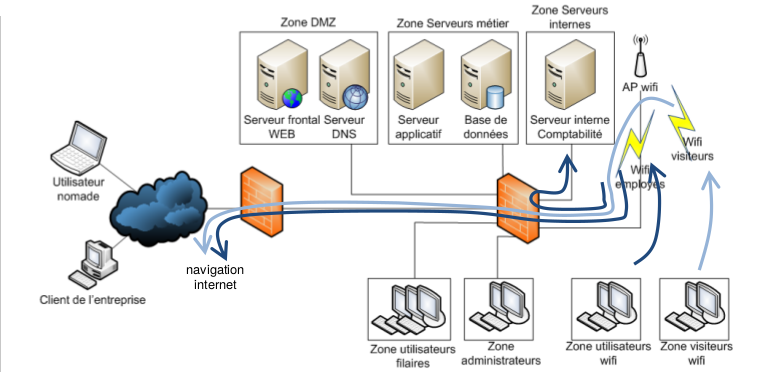
\includegraphics[width=.9\textwidth]{images/reseau_securise.png}
  \caption{Network separated into different zones}
  \label{fig:reseau:securise}
\end{figure}

\end{frame}


\begin{frame}[c]{Questions (1/n)}
  
  \begin{block}{Preparation}
    Prepare a table (on paper) with 1 line and 1 column for each zone
    (so a \(n\times n\) table). On line \(i\), column \(j\), select
    whether the communications from zone \(i\) to zone \(j\) should be
    \(A\) accepted, \(D\) denied, or \(R\) response only. The wifi iis
    considered to be a unique zone. You can also specify a protocol if
    need be.
  \end{block}

  \vfill\pause \small
  
    \begin{center}
    \begin{tabular}{|l|c|c|c|c|c|c|c|}
      \hline
      &Internet&DMZ&App&internal BP&wifi&admin&Ethernet\\\hline
      Internet&&A,web &D&D&R&R&R\\\hline
      DMZ&R& & R &D&R&R&R\\\hline
      BP&D&A&&D&D&R&R\\\hline
      internal BP&D&D&D&&D&R&R\\\hline
      wifi&A&A&D&D&&D&D\\\hline
      admin&A&A&A&A&D& &A\\\hline
      Ethernet&A&A&A&A&D&R& \\\hline
    \end{tabular}
  \end{center}
\end{frame}
\defverbatim[colored]\lstI{%
\begin{lstlisting}[language=bash]
iptables -t nat --flush
iptables -t nat -A POSTROUTING -i eth0 -o eth1 -j MASQUERADE   
\end{lstlisting}
}
\defverbatim[colored]\lstII{%
\begin{lstlisting}[language=bash]
iptables -t nat -A PREROUTING  -p tcp --dport 80  \
-j DNAT --to 172.31.0.23:80
iptables -t nat -A PREROUTING  -p tcp --dport 443  \
-j DNAT --to 172.31.0.23:80   
\end{lstlisting}
}
\defverbatim[colored]\lstIII{%
\begin{lstlisting}[language=bash]
# Accept redirections to the Web server wherever they come from
iptables -A FORWARD  -p tcp --dport 80 -d 172.31.0.23 -j accept
# Default rules
iptables -A FORWARD  -i eth1 -o eth0 -m state --state NEW -j REJECT
iptables -A FORWARD  -i eth1 -o eth0 -m state \
 --state ESTABLISHED,RELATED -j ACCEPT
iptables -A FORWARD  -i eth0 -o eth1  -j ACCEPT
\end{lstlisting}
}
\begin{frame}[c,fragile]{Rules}
  
  \begin{enumerate}
  \item Separate the LAN from Internet with a NAT firewall
    \only<2>{
      \begin{center}
        \lstI
      \end{center}
}
  \item Transfert the http and https requests on port 80 (tcp
    protocol) and 443 (TLS) of the firewall to the Web server at LAN
    address \verb+192.168.1.17+.
    \only<3>{
      \begin{center}
        \lstII
      \end{center}
}
  \item Reject all other communications from the Internet to the LAN,
    but for those (tcp) that are responses to LAN-issued requests
    \only<4>{
      \begin{center}
        \lstIII
      \end{center}
}
  \end{enumerate}

\end{frame}



\subsection{IPTables modules}

\begin{frame}[c]{Modules}
  
  \begin{block}{Context}
    \begin{itemize}
    \item iptables also has a number of modules that can be employed
      for a finer grained access control
    \item they are automatically loaded when used
    \item works like the \texttt{-m state} (m is for module)
    \end{itemize}
  \end{block}

  \vfill

  \begin{block}{Examples (-m name)}
    \begin{description}
    \item[conntrack:] control according to the position in a tcp session
    \item[owner:] Allow to control the output according to the user
      running the application that sends the packet
    \item[limits:] limits the number of packets per second
    \item[recent:] allows to limit the number of packets per origin
      (for DoS attacks)
    \end{description}
  \end{block}

\end{frame}

\section{Firewalls under the Hood}


\begin{frame}[c]{Iptables summary}

  \begin{itemize}
  \item Tables: filter, nat, mangle, \(\ldots\)
  \item Hooks: input, output, forward, \(\ldots\)
    \begin{center}
      \color{red}Each table has a subset of these
    \end{center}
  \item Chains: DAG of rules 
    \begin{center}
      \color{red}attached to hooks
    \end{center}
  \item Rules: set of matches and a judgement/target
    \begin{center}
      \color{red}iptables -A INPUT -s 2.2/16 -d 3/8 -p udp -dport 25 -j DROP
    \end{center}
  \end{itemize}
  
\end{frame}

\begin{frame}[c]{Internal representation}
  
  \begin{block}{Internal storage}
    \begin{itemize}
    \item Rules are represented by structures, with a flexible array for
      matches
    \item Chains represented by structures, with flexible array for rules
    \item Rules are appended at the end of the array
    \end{itemize}
  \end{block}

  \vfill
  \begin{block}{Rule compilation and evaluation}
    \begin{itemize}
    \item Iptables compiles the set of rules into a structure in a
      \texttt{.o} object file, and loads that file into the kernel on a hook
    \item The kernel reads these rules one after the other
    \end{itemize}
  \end{block}

  \vfill
  
  \begin{block}{Consequence}
    \begin{itemize}
    \item The filtering time is linear \textit{wrt} the number of
      rules
    \item No way to jump to another case (\textit{e.g.} if the
      protocol is udp, ignore all tcp rules)
    \end{itemize}
  \end{block}
\end{frame}


\begin{frame}[c]{User mode helper (Linux)}
  
  \begin{block}{Overview}
    \begin{itemize}
    \item Userspace process: called by the kernel upon some condition,
      with a return code processed by the kernel
    \item Communication channel: session key for shared memory, pipe
      (kernel \(\rightarrow\) process, for core dumps)
    \item IPC
    \end{itemize}
  \end{block}

  \vfill

  \begin{block}{Example usage}
    \begin{itemize}
    \item kernel detects a device is plugged in
    \item kernel launches a userspace process (modprobe) to load the
      driver module for that device
    \item Examples: code to put in a kernel module that will call an
      external application
    \end{itemize}
  \end{block}

\end{frame}


\begin{frame}[c]{UMH in the Kernel}

  \begin{center}
    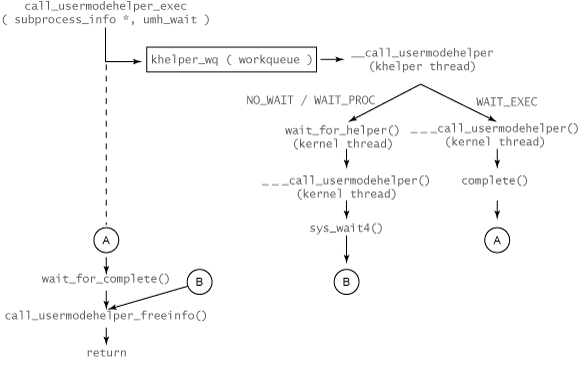
\includegraphics[width=0.9\textwidth]{images/umh-kernel.png}
  \end{center}
  
\end{frame}
\begin{comment}
  When an element is placed onto the khelper_wq, the handler function
  for the work queue is invoked (in this case, __call_usermodehelper),
  which is run through the khelper thread. This function begins by
  dequeuing the subprocess_info structure, which contains all of the
  necessary information for the user-space invocation. The path next
  depends upon the wait variable enumeration. If the requester wants
  to wait for the entire process to finish, including user-space
  invocation (UMH_WAIT_PROC) or not wait at all (UMH_NO_WAIT), then a
  kernel thread is created from the function
  wait_for_helper. Otherwise, the requester simply wants to wait for
  the user-space application to be invoked (UMH_WAIT_EXEC) but not
  complete. In this case, a kernel thread is created for
  ____call_usermodehelper().

  In the wait_for_helper thread, a SIGCHLD signal handler is
  installed, and another kernel thread is created for
  ____call_usermodehelper. But in the wait_for_helper thread, a call
  is made to sys_wait4 to await termination of the
  ____call_usermodehelper kernel thread (indicated by a SIGCHLD
  signal). The thread then performs any necessary cleanup (either
  freeing the structures for UMH_NO_WAIT or simply sending a
  completion notification back to call_usermodehelper_exec().

The function ____call_usermodehelper is where the real work happens
for getting the application started in user space. This function
begins by unblocking all signals and setting the session key ring. It
also installs the stdin pipe (if requested). After a bit more
initialization, the user-space application is invoked through a call
to kernel_execve (from kernel/syscall.c), which includes the
previously defined path, argv list (including the user-space
application name), and environment. When this process is complete, the
thread exits through a call to do_exit().

This process also uses Linux completions, which is a semaphore-like
operation. When the call_usermodehelper_exec function is invoked, a
completion is declared. After the subprocess_info structure is placed
on the khelper_wq, a call is made to wait_for_completion (using the
completion variable as its only argument). Note that this variable is
also stored in the subprocess_info structure as the complete
field. When the child threads want to wake up the
call_usermodehelper_exec function, they call the kernel method
complete, noting the completion variable from the subprocess_info
structure. This call unlocks the function so that it can continue. You
can find the implementation of this API in include/linux/completion.h.

You’ll find more information on the usermode-helper API by following
the links in the resources section on the right.
\end{comment}

\begin{frame}[c,fragile]{UMH in User space (full)}

\begin{lstlisting}[language=C]
static int umh_test( void )
{
  struct subprocess_info *sub_info;
  char *argv[] = { "/usr/bin/logger", "help!", NULL };
  static char *envp[] = {
        "HOME=/",
        "TERM=linux",
        "PATH=/sbin:/bin:/usr/sbin:/usr/bin", NULL };

  sub_info = call_usermodehelper_setup( 
                 argv[0], argv, envp, GFP_ATOMIC );
  if (sub_info == NULL) return -ENOMEM;

  return call_usermodehelper_exec( 
                 sub_info, UMH_WAIT_PROC );
}
\end{lstlisting}
\end{frame}
\begin{frame}[c,fragile]{UMH in User space (easy)}

\begin{lstlisting}[language=C]
static int umh_test( void )
{
  char *argv[] = { "/usr/bin/logger", "help!", NULL };
  static char *envp[] = {
        "HOME=/",
        "TERM=linux",
        "PATH=/sbin:/bin:/usr/sbin:/usr/bin", NULL };

  return call_usermodehelper( 
              argv[0], argv, envp, UMH_WAIT_PROC );
}
\end{lstlisting}
\end{frame}

\begin{frame}[c]{UMH for BPFilter}
  
  \begin{block}{Overview}
    \begin{itemize}
    \item Like loading modules with modproble, loads firewall code instead
    \item Same structures for compatibility with iptables
    \item \textcolor{red}{eBPF} programs are compiled and inserted
      into hooks by userspace programs
    \item Code optimisation by userspace programs (tree instead of
      list)
    \item Generic linux kernel infrastructure: \textcolor{red}{eBPF}
    \end{itemize}
  \end{block}


\end{frame}

\begin{frame}[c,fragile]{Classic BPF}
  
  \begin{block}{BPF}
    \begin{itemize}
    \item \textbf{hooks} on the kernel network processing functions
    \item BPF code is added to these hooks (on function call or return)
    \end{itemize}
  \end{block}

  \vfill

  \begin{block}{Modus Operandi}
    \begin{itemize}
    \item Create a \texttt{RAW} socket (needs to be root)
    \item Add a filter with setsockopt
\begin{lstlisting}[language=C]
sock = socket(PF_PACKET, SOCK_RAW, htons(ETH_P_ALL))
...
setsockopt(sock, SOL_SOCKET, SO_ATTACH_FILTER, ...)
\end{lstlisting}
    \end{itemize}
  \end{block}

  \vfill

  \begin{block}{Usage}
    \begin{itemize}
    \item iptables
    \item libpcap (at ethernet/layer 2 level)
    \item tcpdump, wireshark
    \end{itemize}
  \end{block}

\end{frame}

\begin{frame}[c]{Extended BPF}

  \begin{block}{Extension}
    \begin{itemize}
    \item Possibility to attach BPF to \textcolor{red}{any} kernel
      function
    \item More generic code (some loops are possible)
    \item Only iptables does not use it, actually
    \end{itemize}
  \end{block}
  
  \vfill

  \begin{block}{Applications}
    \begin{itemize}
    \item Add code to system calls to monitor applications
    \item Traffic shaping/Traffic control
    \item Sandbox applications
    \item Sandbox protocols: \texttt{xt\_bpf} iptables module
    \end{itemize}
  \end{block}

  \vfill

  \begin{center}
    \textcolor{red}{Recent development, no bounds in sight}
  \end{center}
\end{frame}



\begin{frame}[c]{The eBPF Revolution}
  \framesubtitle{\url{https://ebpf.io/}}
  
  \begin{block}{extended BPF}
    \begin{itemize}
    \item More generic language (BPF now called \emph{classic BPF})
    \item Bounded termination of programs has to be proved
    \item Allows \textit{e.g.} implementation of cryptographic
      protocols within the kernel
      \begin{center}
        Falco (monitor), Cilium (Security within the stack for Kubernetes)
      \end{center}
    \end{itemize}
  \end{block}

  \vfill

  \begin{block}{More hooks}
    \begin{itemize}
    \item Hooks are now on all system calls
    \item Allows control, monitoring, and tracing of all applications
      \begin{center}
        Katran (traffic control), bpftrace, ply (for embedded systems)
      \end{center}
    \end{itemize}
  \end{block}

\end{frame}


\end{reveals}

\end{document}